\author{'Josef Stieg'}

\subsection{Entwicklungsumgebung}
Für die Entwicklung des Backends wurde die Entwicklungsumgebung \textbf{IntelliJ IDEA} aus der \textbf{JetBrains Toolbox} verwendet. Die Wahl fiel auf IntelliJ aus mehreren Gründen, die sowohl auf der Erfahrung des Entwicklerteams als auch auf den zahlreichen Vorteilen dieser integrierten Entwicklungsumgebung (IDE) beruhen.  

Ein entscheidender Faktor für die Nutzung von IntelliJ ist, dass das Entwicklerteam die JetBrains Toolbox, und damit auch IntelliJ IDEA, regelmäßig im Schulalltag verwendet. Durch diese häufige Nutzung war das Team bereits mit der Benutzeroberfläche, den Funktionen und der Konfiguration der IDE vertraut, was den Einstieg in die Entwicklung deutlich erleichterte. Diese Vertrautheit reduzierte die Lernkurve und ermöglichte eine produktive Arbeitsweise von Beginn an.  

Darüber hinaus bietet IntelliJ IDEA zahlreiche Vorteile, die es zu einer ausgezeichneten Wahl für die Backend-Entwicklung machen: 

\begin{itemize}
    \item 
    \textbf{Umfassende Unterstützung für Java und Frameworks: }
    IntelliJ IDEA ist speziell auf die Java-Entwicklung zugeschnitten und bietet erstklassige Unterstützung für Frameworks wie Quarkus, Spring und Jakarta EE. Dadurch werden Konfigurationsaufgaben erleichtert, und die Arbeit mit modernen Frameworks wird durch eingebaute Tools und Assistenten optimiert.

    \item 
    \textbf{Intelligente Code-Navigation:} 
    Mit Funktionen wie Code-Vervollständigung, Refactoring-Tools und schneller Navigation durch Projekte bietet IntelliJ eine hochproduktive Umgebung, die den Entwicklungsprozess beschleunigt und Fehler reduziert.  

    \item 
    \textbf{Einfache Integration von Plugins: }
    IntelliJ unterstützt eine Vielzahl von Plugins, die sich nahtlos in die Entwicklungsumgebung integrieren lassen. Dadurch können zusätzliche Tools und Technologien, die im Projekt benötigt werden, schnell eingebunden werden.  

    \item 
    \textbf{Integrierte Tools:} 
    IntelliJ bietet zahlreiche integrierte Werkzeuge wie einen Version-Control-Client (z. B. für Git), eine Datenbank-Integration und ein leistungsstarkes Debugging-System. Diese Funktionen machen externe Tools oft überflüssig und ermöglichen ein konzentriertes Arbeiten innerhalb der IDE. 

    \item 
    \textbf{Benutzerfreundlichkeit:} 
    Die intuitive Benutzeroberfläche, anpassbare Einstellungen und umfangreiche Dokumentation machen IntelliJ IDEA zu einer leicht zugänglichen Entwicklungsumgebung – sowohl für Einsteiger als auch für erfahrene Entwickler. 

    \item 
    \textbf{Leistungsfähigkeit und Stabilität:} 
    IntelliJ IDEA ist bekannt für seine zuverlässige Leistung, selbst bei großen Projekten mit komplexer Codebasis.  
\end{itemize}

Zusätzlich bietet die JetBrains Toolbox den Vorteil, dass alle relevanten JetBrains-Tools zentral verwaltet werden können. So bleibt die Entwicklungsumgebung stets aktuell, und der Zugriff auf andere Tools wie DataGrip oder PhpStorm wird erleichtert, falls diese im Projekt benötigt werden.  

Die Kombination aus der Vertrautheit des Teams mit der Umgebung, der leistungsstarken Unterstützung für Java und modernen Frameworks sowie den zahlreichen integrierten Werkzeugen machte IntelliJ IDEA zur idealen Wahl für die Entwicklung des Backends.

\begin{figure}[H]
    \centering
    
\includegraphics[width=0.25\linewidth]{pics//Backend/JetBrains_IntelliJ_IDEA_Icon.png}
    \caption{Intellij IDEA - Jetbrains}
    \label{fig:intelij}
\end{figure}

\newpage

\subsection{Model}

Im Melius-Backend erfolgt die Erstellung und Verwaltung aller Datenbanktabellen unter Zuhilfenahme der Jakarta Persistence API (JPA) in Kombination mit Hibernate als Object-Relational Mapping (ORM)-Framework. Dies impliziert, dass jede in der Anwendung definierte Java-Entitätsklasse einer eigenen Tabelle in der Datenbank entspricht.

Dies hat den Vorteil, dass die Verwaltung der Daten erheblich vereinfacht wird, da Entwickler nicht direkt mit SQL-Abfragen arbeiten müssen, sondern auf objektorientierte Weise mit den Daten interagieren können.

Durch diese ORM-Technologie können Datenbankoperationen wie Erstellen, Lesen, Aktualisieren und Löschen (CRUD-Operationen) direkt über Java-Klassen durchgeführt werden. Hibernate übernimmt dabei automatisch die Zuordnung der Java-Objekte zu den entsprechenden Tabellen und Spalten, sodass eine enge Integration zwischen der Anwendung und der Datenbank entsteht.

\begin{figure}[H]
    \centering
    
\includegraphics[width=0.5\linewidth]{pics/Backend/Entitäten/entities.png}
    \caption{Enitity - Klassen}
    \label{fig:entities}
\end{figure}

\subsubsection{Beispiele}

\subsubsection{Portfolio - Klasse}
Die Portfolio-Klasse konstituiert das zentrale Element der Datenstruktur im Backend. Sie fungiert als Hauptentität und verweist auf nahezu alle anderen Entitäten, die auf der Portfolio-Seite dargestellt werden. In dieser Funktion verknüpft sie verschiedene Datenbereiche miteinander und ermöglicht eine strukturierte Verwaltung sowie eine effiziente Abfrage der relevanten Informationen.

\subsubsection{Annotationen}

\subsubsection{@Id}
Diese Annotation kennzeichnet das Primärschlüsselfeld der Entität.
In dieser Klasse fehlt jedoch die @GeneratedValue-Annotation, die für die automatische Generierung eines Primärschlüssels sorgen könnte.

\subsubsection{@OneToOne}
Diese Annotation beschreibt eine 1:1-Beziehung zwischen der Portfolio-Entität und einer anderen Entität.
\begin{figure}[H]
    \centering
    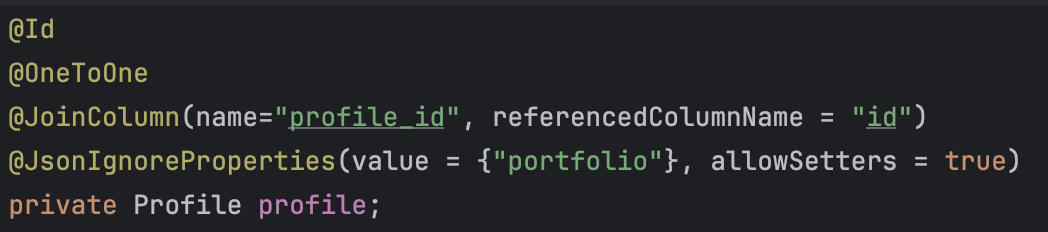
\includegraphics[width=0.75\linewidth]{pics/Backend/Entitäten/one-to-one-profile.png}
    \caption{OneToOne}
    \label{fig:entities}
\end{figure}

\begin{itemize}
    \item
    Diese Beziehung bedeutet, dass jedes Portfolio genau ein Profile-Objekt besitzt.

    \item
\begin{verbatim}
@JoinColumn(name="profile_id", referencedColumnName = "id"):
\end{verbatim}
profileId ist der Fremdschlüssel in der Portfolio-Tabelle,
der auf die id-Spalte der Profile-Tabelle verweist.


    \item
\begin{verbatim}
@JsonIgnoreProperties(value = {"portfolio"}, allowSetters = true):
\end{verbatim}
stellt sicher, dass bei JSON-Serialisierung rekursive Referenzen
zwischen Portfolio und Profile vermieden werden.


\end{itemize}

\begin{figure}[H]
    \centering
    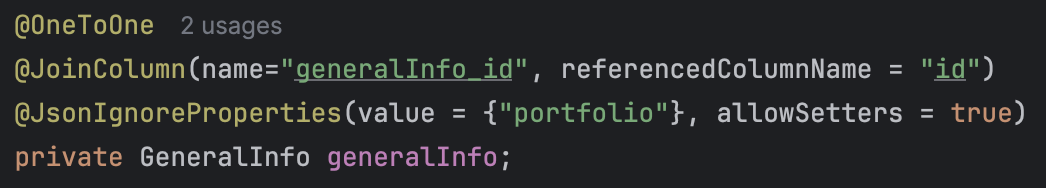
\includegraphics[width=0.75\linewidth]{pics/Backend/Entitäten/one-to-one-general.png}
    \caption{OneToOne}
    \label{fig:entities}
\end{figure}


\subsubsection{@OneToMany}
Diese Annotation beschreibt eine 1:n-Beziehung, bei der ein Portfolio mehrere abhängige Entitäten besitzt.

\begin{figure}[H]
    \centering
    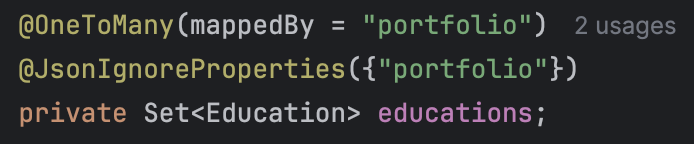
\includegraphics[width=0.75\linewidth]{pics/Backend/Entitäten/one-to-many.png}
    \caption{OneToMany}
    \label{fig:entities}
\end{figure}


\begin{itemize}
    \item
    Ein Portfolio kann mehrere Education-Einträge haben.

    \item
    \textbf{mappedBy = "portfolio"} zeigt, dass die Education-Entität eine portfolio-Referenz besitzt.

    \item
\begin{verbatim}
@JsonIgnoreProperties({"portfolio"}):
\end{verbatim}
verhindert rekursive JSON-Serialisierung.


\end{itemize}

\textbf{Weitere 1:n-Beziehungen:}
\begin{itemize}
    \item
    Set<WorkExperience> workExperiences

    \item
    Set<KnownLanguage> knownLanguages

    \item
    Set<ProgrammingKnowledge> programmingKnowledges

    \item
    Set<SoftwareKnowledge> softwareKnowledges
\end{itemize}

Diese Beziehungen ermöglichen, dass ein Portfolio mehrere berufliche Erfahrungen, Sprachen, Programmierkenntnisse oder Softwarekenntnisse speichern kann.

\subsubsection{@ManyToMany}
Diese Annotation beschreibt eine n:m-Beziehung, bei der mehrere Portfolios mehrere Eigenschaften (Characteristic) haben können.

\begin{figure}[H]
    \centering
    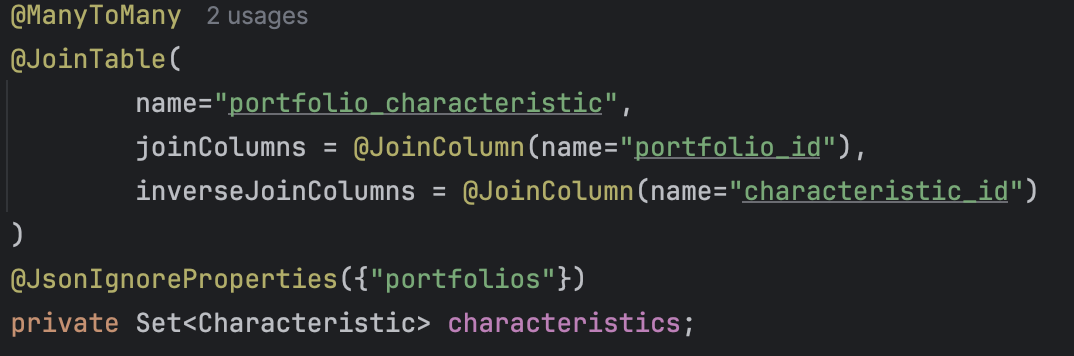
\includegraphics[width=0.75\linewidth]{pics/Backend/Entitäten/many-to-many.png}
    \caption{ManyToMany}
    \label{fig:entities}
\end{figure}


\begin{itemize}
    \item
    Dies bedeutet, dass eine separate Join-Tabelle (portfolio\_characteristic) existiert,
    die die Verknüpfung zwischen Portfolio und Characteristic speichert.

    \item
\begin{verbatim}
joinColumns = @JoinColumn(name="portfolio_id"):
\end{verbatim}
Verweist auf die portfolio_id-Spalte in der Join-Tabelle.


    \item
\begin{verbatim}
inverseJoinColumns = @JoinColumn(name="characteristic_id"):
\end{verbatim}
Verweist auf die characteristic_id-Spalte.

\end{itemize}

\subsubsection{Zusätzliche String-Felder}
Die Klasse enthält mehrere String-Attribute für Positionen wie:
private String generalInfoPosition;
private String educationsPosition;
private String workExperiencesPosition;
Diese Felder werden verwendet, um die Spalten - Positionen der einzelnen Boxen im Portfolio zu speichern.

\begin{figure}[H]
    \centering
    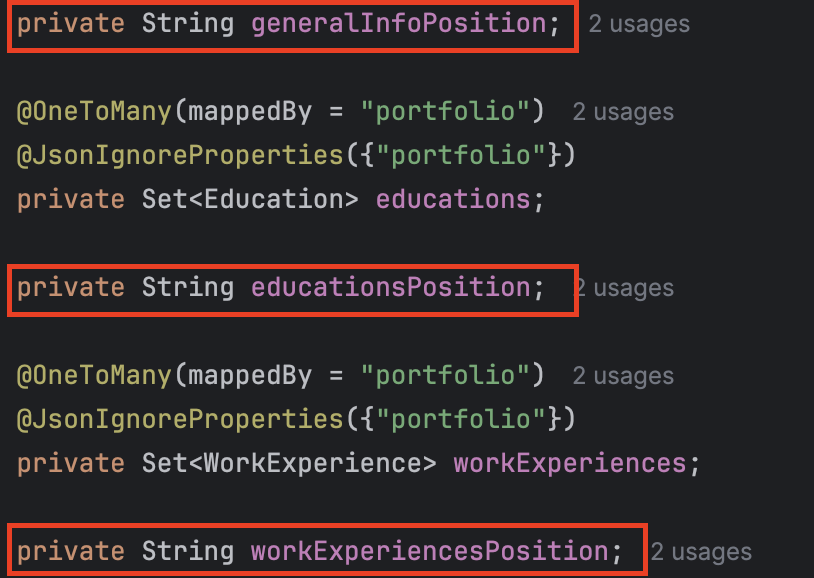
\includegraphics[width=0.75\linewidth]{pics/Backend/Entitäten/portfolio-strings.png}
    \caption{Portfolio - Strings}
    \label{fig:entities}
\end{figure}

\newpage

\subsection{Repository}
Zur Gewährleistung einer effizienten Verwaltung und Interaktion mit den verschiedenen Entity-Klassen wurde für nahezu jede Entitätsklasse eine entsprechende Repository-Klasse implementiert.Die Repository-Klassen fungieren als Schnittstelle zwischen der Anwendung und der Datenbank und ermöglichen grundlegende CRUD-Operationen (Create, Read, Update, Delete) sowie komplexe Datenabfragen.

Die Verwendung von Spring Data JPA ermöglicht die Durchführung vieler dieser Abfragen ohne umfangreiche manuelle SQL-Statements, da Spring Data automatisch Methoden zur Datenverarbeitung bereitstellt. Zudem lassen sich individuelle Abfragen mithilfe von JPQL (Java Persistence Query Language) oder der Criteria API definieren, um spezifische Datenanforderungen effizient umzusetzen.

\begin{figure}[H]
    \centering
    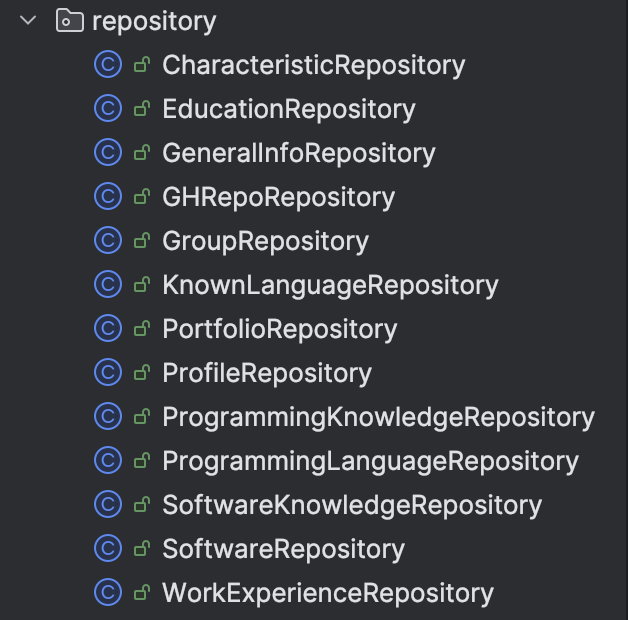
\includegraphics[width=0.5\linewidth]{pics/Backend/Repositories/Repos.png}
    \caption{Repository - Klassen}
    \label{fig:entities}
\end{figure}

\subsubsection{Beispiele}

\subsubsection{ProfileRepository - Klasse}
Die ProfileRepository-Klasse spielt eine zentrale Rolle in der Verwaltung von Benutzerprofilen innerhalb der Anwendung. Sie ist für grundlegende CRUD-Operationen (Erstellen, Lesen, Aktualisieren und Löschen) von Profilen verantwortlich und stellt sicher, dass diese effizient in der Datenbank gespeichert und verwaltet werden.

Neben diesen Standardfunktionen übernimmt die ProfileRepository-Klasse auch wichtige Überprüfungen und Sicherheitsmaßnahmen. Beispielsweise wird bei einem Benutzer-Login das eingegebene Passwort mit dem in der Datenbank gespeicherten Hash-Wert verglichen, um die Identität des Nutzers zu bestätigen. Darüber hinaus wird bei der Registrierung neuer Nutzer überprüft, ob bereits ein Profil mit der gleichen E-Mail-Adresse existiert, um Doppelregistrierungen zu verhindern und die Datenintegrität zu gewährleisten.

Dank dieser Funktionen trägt das Repository maßgeblich zur Sicherheit, Datenkonsistenz und Benutzerverwaltung innerhalb der Anwendung bei. Es ermöglicht eine reibungslose Interaktion mit der Datenbank und bildet eine essenzielle Schnittstelle zwischen Backend-Logik und Datenpersistenz.

\subsubsection{Annotationen}

\subsubsection{@ApplicationScoped}
Die Annotation @ApplicationScoped, die aus Jakarta CDI (Contexts and Dependency Injection) stammt, gewährleistet, dass eine Klasse während der gesamten Laufzeit der Anwendung lediglich einmal instanziiert wird. Dies impliziert, dass sämtliche Beans, welche diese Klasse verwenden, auf die identische Instanz zugreifen und folglich ein Singleton-Verhalten erzielen.In Bezug auf die ProfileRepository-Klasse resultiert daraus eine Vielzahl an Vorteilen. Da das Repository für den Zugriff auf die Datenbank zuständig ist, sorgt @ApplicationScoped dafür, dass nicht bei jeder Anfrage eine neue Instanz erstellt wird, sondern alle Datenbankoperationen über eine einzige, wiederverwendbare Instanz laufen.Dies verbessert die Effizienz, da weniger Ressourcen für das Erstellen neuer Objekte verbraucht werden. Darüber hinaus bleibt der Zustand der Bean während der gesamten Laufzeit der Anwendung erhalten. Dies kann sich beispielsweise positiv auf Caching-Mechanismen oder optimierte Datenbankverbindungen auswirken.
\begin{figure}[H]
    \centering
    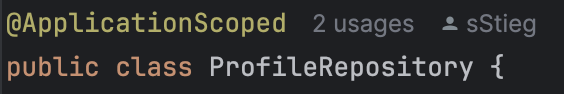
\includegraphics[width=0.75\linewidth]{pics/Backend/Repositories/applicationscoped.png}
    \caption{ApplicationScoped}
    \label{fig:entities}
\end{figure}

\subsubsection{@Transactional}
Der Einsatz von @Transactional in den Methoden addProfile und updateProfile gewährleistet folglich die Aufrechterhaltung der Datenkonsistenz und verhindert das Auftreten inkonsistenter oder unvollständiger Datenbankzustände. Im Falle eines Fehlers während der Ausführungsphase der Methoden wird die gesamte Transaktion automatisch zurückgesetzt, wodurch fehlerhafte oder unvollständige Änderungen in der Datenbank verhindert werden.

\begin{itemize}
    \item 
    \textbf{addProfile(Profile profile)}
    Diese Methode prüft zunächst, ob bereits ein Profil mit der angegebenen E-Mail existiert. Falls nicht, wird das neue profile mit entityManager.persist(profile) in die Datenbank eingefügt. Sollte jedoch bereits ein Profil existieren, wird eine BadRequestException ausgelöst. Durch @Transactional wird sichergestellt, dass die gesamte Methode entweder komplett erfolgreich durchläuft oder im Fehlerfall keine Teildaten gespeichert werden.

    \item
    \textbf{updateProfile(Profile profile)}
    Hier wird das übergebene profile mit entityManager.merge(profile) aktualisiert. Auch diese Methode ist mit @Transactional versehen, wodurch sichergestellt wird, dass alle Änderungen an der Datenbank entweder vollständig übernommen oder – falls ein Fehler auftritt – zurückgesetzt werden.

\end{itemize}

\begin{figure}[H]
    \centering
    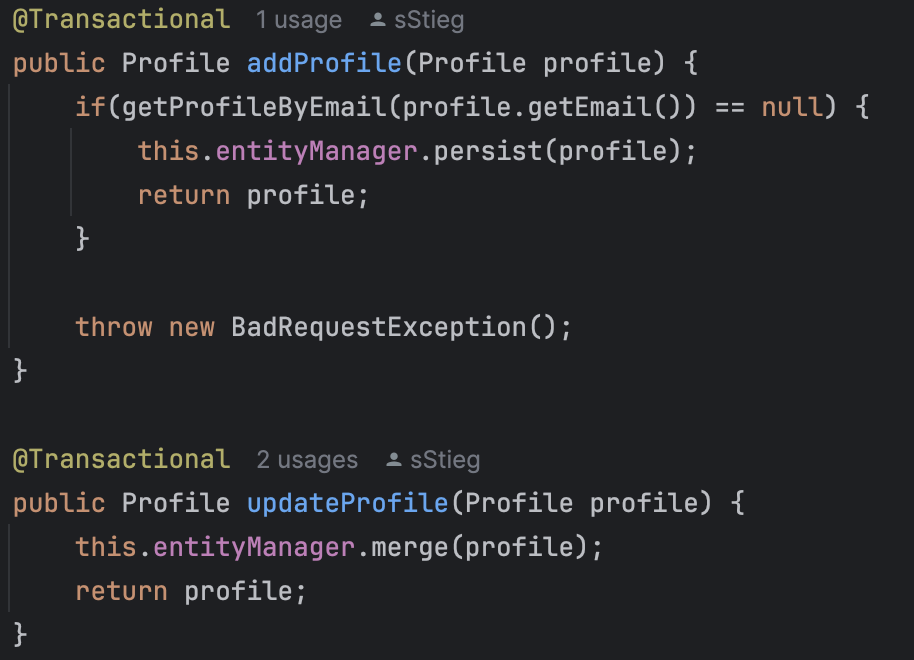
\includegraphics[width=0.75\linewidth]{pics/Backend/Repositories/Transactional.png}
    \caption{Transactional}
    \label{fig:entities}
\end{figure}

\subsubsection{Wichtige Funktionen}

\subsubsection{addProfile}
Die Methode `addProfile()` dient dazu, ein neues Profil in die Datenbank zu speichern. Bevor das Profil jedoch eingefügt wird, erfolgt eine Überprüfung, ob bereits ein anderes Profil mit derselben E-Mail-Adresse existiert. Dadurch wird verhindert, dass sich mehrere Benutzer mit identischen E-Mail-Adressen registrieren, was die Datenkonsistenz und Eindeutigkeit der Benutzerprofile sicherstellt.

\begin{figure}[H]
    \centering
    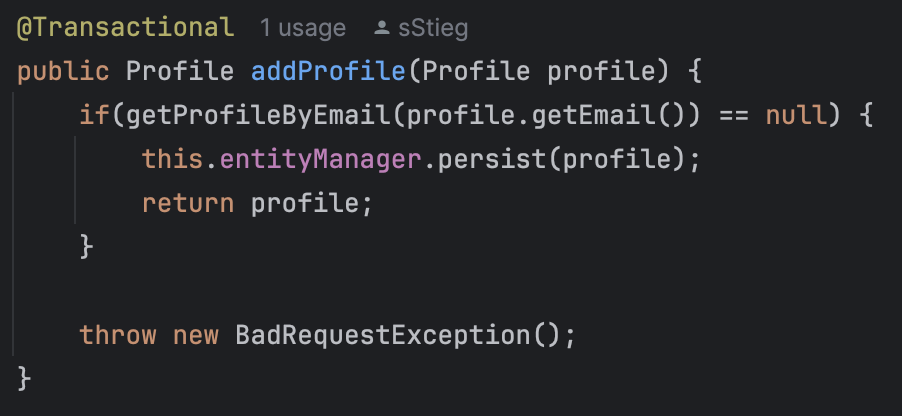
\includegraphics[width=0.75\linewidth]{pics/Backend/Repositories/addProfile.png}
    \caption{addProfile}
    \label{fig:entities}
\end{figure}

\subsubsection{checkProfile}
Die Methode "checkProfile()" findet Anwendung im Rahmen des Autorisierungsprozesses für ein Login. Im ersten Schritt wird das Profil des Nutzers anhand der von ihm eingegebenen E-Mail-Adresse aus der Datenbank abgerufen. Daraufhin erfolgt ein Abgleich zwischen dem von dem Nutzer eingegebenen Passwort und dem im Profil gespeicherten Passwort. Diese Methode wird nicht nur beim eigentlichen Login-Prozess verwendet, sondern auch bei jedem Neuladen der Seite, um die Authentifizierung des Nutzers sicherzustellen.

\begin{figure}[H]
    \centering
    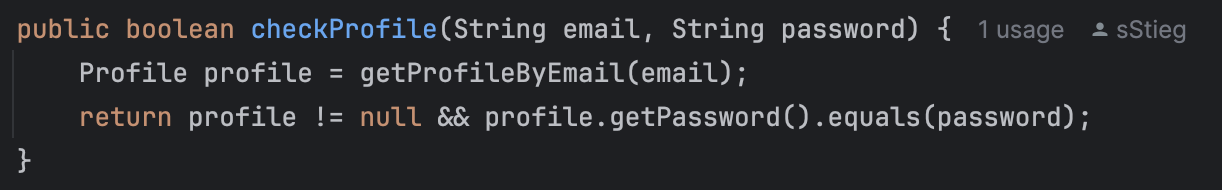
\includegraphics[width=0.75\linewidth]{pics/Backend/Repositories/checkProfile.png}
    \caption{checkProfile}
    \label{fig:entities}
\end{figure}

\subsubsection{getProfileByEmail}
Die Methode "getProfileByEmail()" nimmt eine signifikante Rolle im Kontext der Verwaltung von Benutzerprofilen ein. Sie wird unter anderem bei der Erstellung eines neuen Profils eingesetzt, um die Existenz doppelter Profile mit identischer E-Mail-Adresse zu verhindern. Dies dient dazu, die Vergabe identischer Anmeldedaten an mehrere Benutzer zu unterbinden. 

Darüber hinaus ist diese Funktion von entscheidender Bedeutung für den Login-Prozess. Da beim Einloggen die eindeutige ID des Profils nicht bekannt ist, sondern lediglich die E-Mail-Adresse des Nutzers vorliegt, kann das zugehörige Profil nicht direkt über den Primärschlüssel mit entityManager.find() ermittelt werden. Stattdessen durchsucht getProfileByEmail() die gespeicherten Profile nach der angegebenen E-Mail-Adresse und gibt das entsprechende Profil zurück. Diese Vorgehensweise gewährleistet, dass die Anmeldeinformationen korrekt sind und die Authentifizierung des korrekten Nutzers sichergestellt werden kann.

\begin{figure}[H]
    \centering
    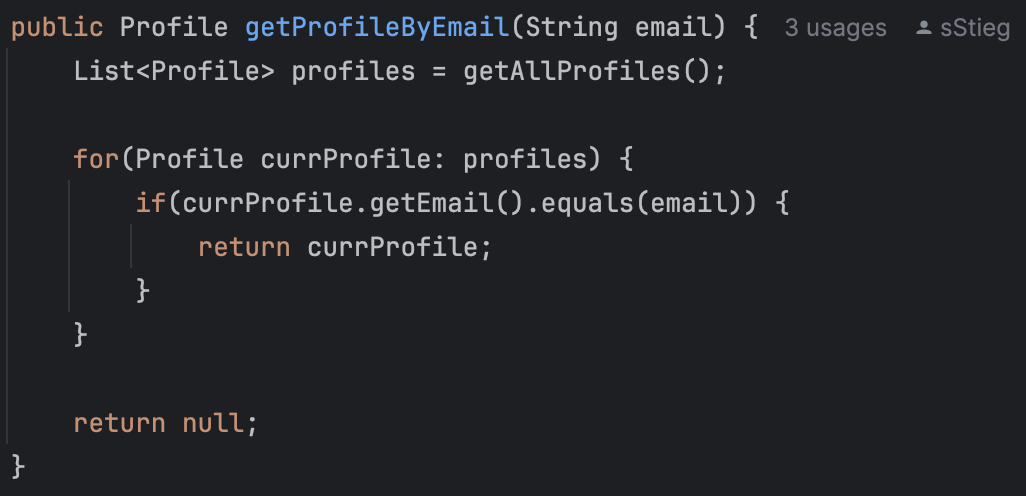
\includegraphics[width=0.75\linewidth]{pics/Backend/Repositories/getProfileByEmail.png}
    \caption{getProfileByEmail}
    \label{fig:entities}
\end{figure}

\subsection{Resource}
Die Resource-Klassen nehmen eine zentrale Rolle in der Kommunikation zwischen dem Frontend und dem Backend ein. Sie fungieren als Vermittler, indem sie über REST-Endpunkte Anfragen aus dem Frontend entgegennehmen und die entsprechenden Daten aus der Datenbank abrufen oder speichern.

Jede Resource-Klasse ist dabei speziell für eine bestimmte Entität zuständig und bildet eine Schnittstelle zu einem zugehörigen Repository. Dies gewährleistet, dass sämtliche Datenbankoperationen effizient und strukturiert durchgeführt werden.Das Frontend kann über die definierten Endpunkte beispielsweise neue Einträge erstellen, bestehende Daten abrufen, aktualisieren oder löschen.

\begin{figure}[H]
    \centering
    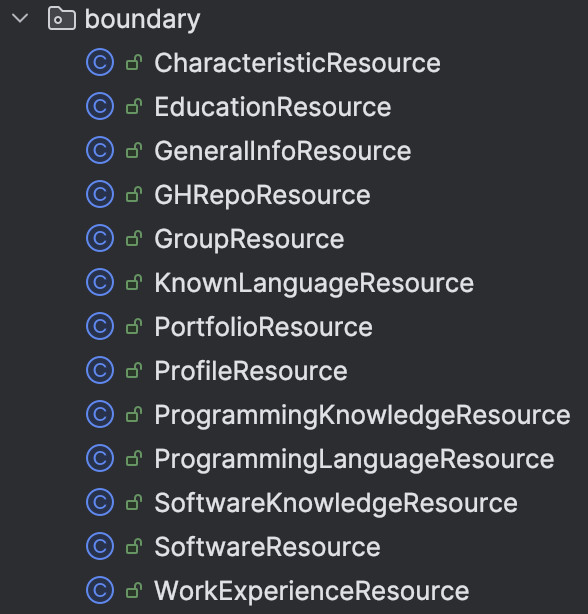
\includegraphics[width=0.5\linewidth]{pics/Backend/Resource/Resources.png}
    \caption{Resource - Klassen}
    \label{fig:entities}
\end{figure}

\subsubsection{Beispiele}

\subsubsection{ProfileResource - Klasse}
Die ProfileResource-Klasse fungiert als zentrale Schnittstelle zwischen dem Frontend und den Datenbankoperationen, die mit den Profilen assoziiert sind. Sie stellt verschiedene REST-Endpunkte bereit, über die das Frontend mit dem Backend kommunizieren kann.

Mittels dieser Endpunkte können unterschiedliche Aktionen ausgeführt werden, wie beispielsweise das Erstellen, Abrufen und Aktualisieren von Profilen in der Datenbank. Die Klasse nutzt dazu Methoden des ProfileRepositorys, um die gewünschten Datenbankabfragen effizient durchzuführen.

Die ProfileResource-Klasse gewährleistet eine klare Trennung zwischen der Präsentations- und der Datenzugriffsschicht und ermöglicht eine strukturierte und sichere Verwaltung der Profildaten.

\subsubsection{Annotationen}

\subsubsection{@Path}
Die @Path-Annotation stellt eine zentrale Annotation in Jakarta RESTful Web Services (JAX-RS) dar. Ihre Funktion besteht in der Festlegung einer URI-Ressource (Uniform Resource Identifier) für eine bestimmte Klasse oder Methode. Somit definiert sie den Endpunkt, unter dem eine bestimmte Ressource oder Funktionalität über eine HTTP-Anfrage erreichbar ist.

\begin{figure}[H]
    \centering
    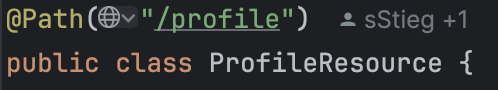
\includegraphics[width=0.5\linewidth]{pics/Backend/Resource/path-class.png}
    \caption{Path - Klasse}
    \label{fig:entities}
\end{figure}

\begin{figure}[H]
    \centering
    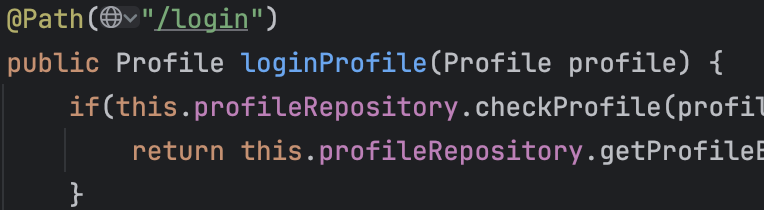
\includegraphics[width=0.6\linewidth]{pics/Backend/Resource/path-method.png}
    \caption{Path - Methode}
    \label{fig:entities}
\end{figure}

\subsubsection{@Produces}

Die @Produces-Annotation in Jakarta RESTful Web Services (JAX-RS) wird verwendet, um anzugeben, in welchem Format eine Methode eine Antwort zurückgibt. Sie definiert also den MIME-Typ (z. B. JSON oder XML), den der Server an den Client sendet. Wird diese Annotation in einer REST-API-Methode verwendet, stellt sie sicher, dass die zurückgegebenen Daten in einem bestimmten Format vorliegen. Beispielsweise kann @Produces(MediaType.APPLICATION\_JSON) verwendet werden, um sicherzustellen, dass die Antwort als JSON formatiert ist. Dies ist besonders nützlich, da moderne Webanwendungen oft JSON als Standardformat für den Datenaustausch nutzen. Wenn keine @Produces-Annotation angegeben ist, entscheidet der Server anhand der Standardkonfiguration oder der Anfrage des Clients, welches Format zurückgegeben wird.

\begin{figure}[H]
    \centering
    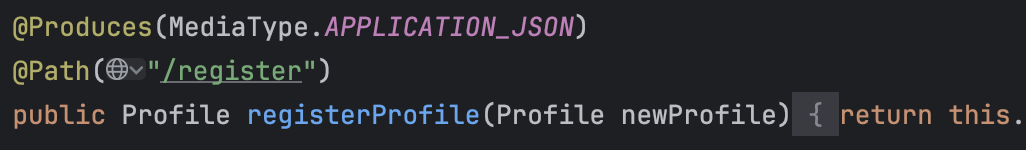
\includegraphics[width=0.75\linewidth]{pics/Backend/Resource/produces.png}
    \caption{Produces}
    \label{fig:entities}
\end{figure}

\subsubsection{@Consumes}

Die @Consumes-Annotation in Jakarta RESTful Web Services (JAX-RS) spezifiziert das Datenformat, welches von einer REST-API-Methode unterstützt wird. Demnach definiert sie die MIME-Typen, die von der Methode verarbeitet werden können. So impliziert @Consumes(MediaType.APPLICATION\_JSON) die Akzeptanz von Anfragen, die mit JSON-Daten angereichert sind. Diese Annotation erweist sich insbesondere dann als vorteilhaft, wenn der Server strukturierte Daten, beispielsweise aus einer Webanwendung oder einer mobilen Applikation, erhält und diese verarbeitet, bevor sie in die Datenbank gespeichert oder weiterverarbeitet werden.Wird @Consumes nicht angegeben, entscheidet der Server anhand der Standardkonfiguration oder der Anfrage des Clients, welches Format akzeptiert wird.

\begin{figure}[H]
    \centering
    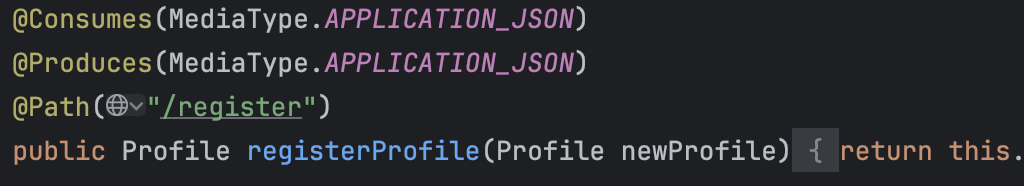
\includegraphics[width=0.75\linewidth]{pics/Backend/Resource/consumes.png}
    \caption{Consumes}
    \label{fig:entities}
\end{figure}

\subsection{Docker-Compose}

Um die Datenbank für Melius zu starten, wird ein docker-compose.yaml-File verwendet, das es ermöglicht, die benötigten Dienste einfach zu konfigurieren und zu starten. In diesem Fall definiert die Datei zwei Hauptservices: Adminer und PostgreSQL.

Der Adminer-Service verwendet das Docker-Image adminer und stellt eine Weboberfläche bereit, über die die PostgreSQL-Datenbank verwaltet werden kann. Der Service wird so konfiguriert, dass er immer neu startet, falls er ausfällt, und ist unter dem Port 5431 zugänglich, der auf den internen Port 8080 des Adminer-Containers weitergeleitet wird.

Der PostgreSQL-Service verwendet das Docker-Image postgres:16-alpine und stellt die tatsächliche Datenbank für Melius bereit. Auch dieser Service wird so konfiguriert, dass er im Falle eines Ausfalls immer neu startet. Die PostgreSQL-Datenbank wird unter dem Standardport 5432 betrieben, das auf den gleichen Port des Hosts weitergeleitet wird. Die volumes-Direktive sorgt dafür, dass die Daten persistent gespeichert werden, indem sie ein Verzeichnis auf dem Host (./data/postgres) mit dem internen Verzeichnis der Datenbank verbindet. Dadurch bleiben die Daten auch nach dem Neustart des Containers erhalten.

Zudem werden Umgebungsvariablen gesetzt, darunter POSTGRES\_PASSWORD, das für den Zugang zur Datenbank verwendet wird, sowie PGDATA, das den Speicherort der Datenbankdateien innerhalb des Containers festlegt. Schließlich wird der Container so konfiguriert, dass er mit den vom System definierten UID und GID läuft, um Berechtigungsprobleme zu vermeiden, was besonders in Teamumgebungen wichtig sein kann, in denen unterschiedliche Benutzer auf die Docker-Container zugreifen.

\begin{figure}[H]
    \centering
    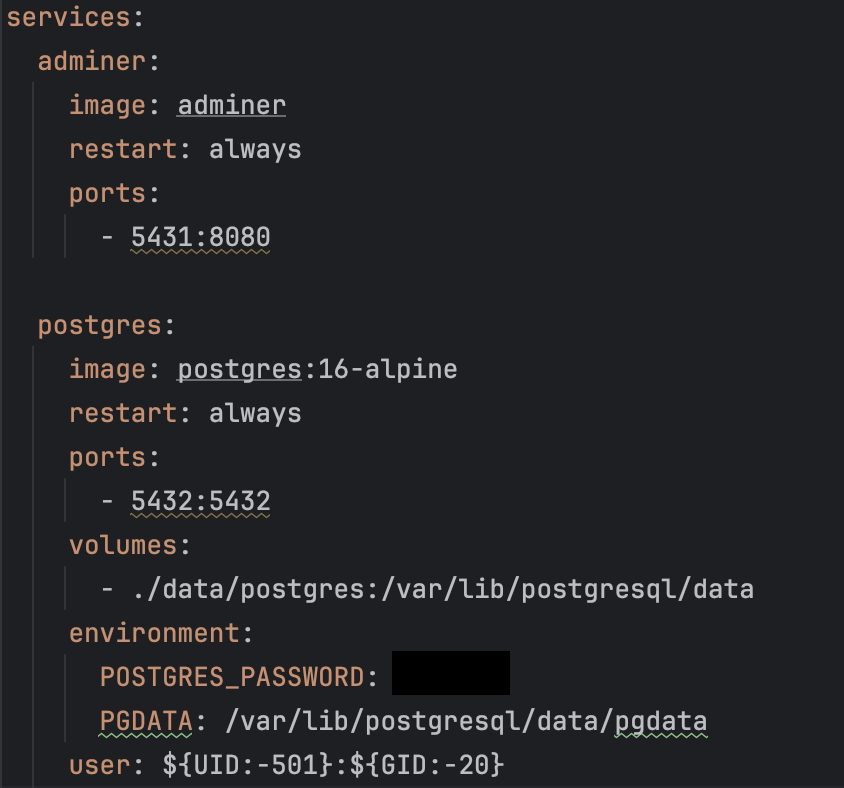
\includegraphics[width=0.75\linewidth]{pics/Backend/docker-compose.png}
    \caption{Docker - Compose}
    \label{fig:entities}
\end{figure}

\subsection{Verwendungen im Frontend}

Das Frontend wurde mit Angular entwickelt, weshalb für alle Backend-Anfragen der HTTPClient genutzt wird. Ähnlich wie bei den Resource-Klassen im Backend, wird für jede Entität ein eigener Service im Frontend verwendet, um die entsprechenden Daten zu verwalten und mit dem Backend zu kommunizieren.

\subsubsection{HttpClient}

Der HttpClient von Angular ist ein Service, der es ermöglicht, HTTP-Anfragen zu stellen, um mit externen APIs oder Backend-Servern zu kommunizieren. Er basiert auf dem RxJS-Bibliothek und bietet eine einfache Möglichkeit, asynchrone Anfragen zu stellen, Daten zu empfangen und darauf zu reagieren.

Der HttpClient unterstützt verschiedene HTTP-Methoden wie GET, POST, PUT, DELETE und PATCH und verarbeitet die Antworten in Form von Observables, was bedeutet, dass er auf die Antwort warten kann, ohne den UI-Thread zu blockieren. Durch die Verwendung von Observables können Entwickler einfach mit den zurückgegebenen Daten arbeiten, Fehler behandeln und auf den Status der Anfrage reagieren (z. B. Erfolg oder Fehler).

\begin{figure}[H]
    \centering
    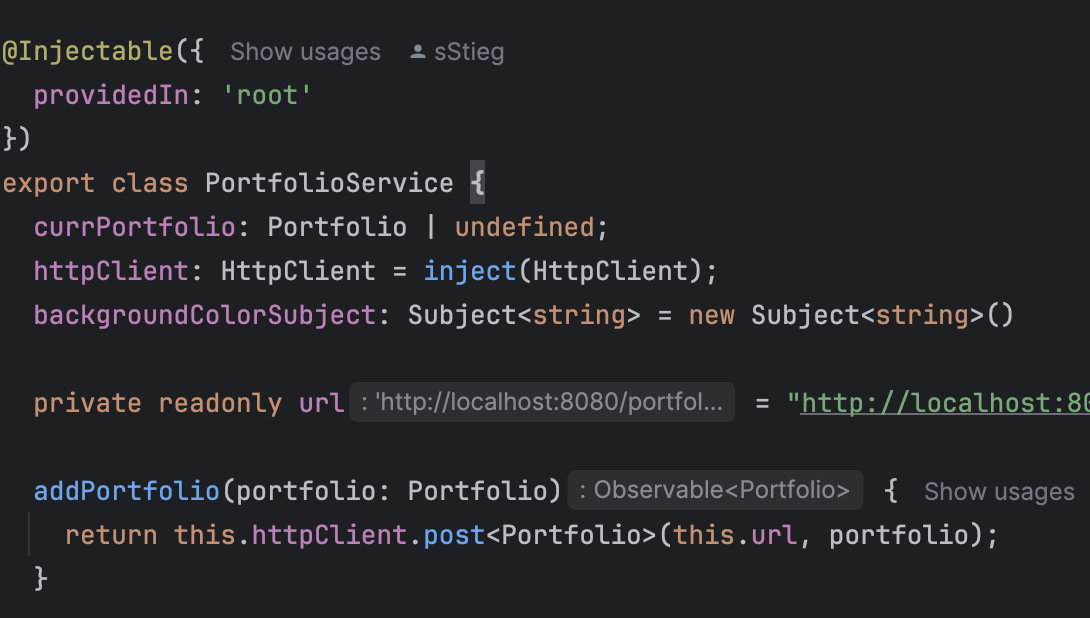
\includegraphics[width=0.75\linewidth]{pics/Backend/Verwendungen/httpclient-beispiel.png}
    \caption{Docker - Compose}
    \label{fig:entities}
\end{figure}
